%!TEX root = ../main.tex

\section{3D Regions}
\label{section:3d_regions}

When we consider moving regions of fixed shape in three dimensions, some of the ideas and concepts used for 2D regions can be reused. For example, when we want to represent a moving region in a compact way, the technique of using the transformation between the instants can be reused. A 3D transformation is, just as in 2D, the combination of a translation and a rotation, but the translation now has three degrees of freedom instead of two, and the rotation also has three degrees of freedom instead of one.

The most important operation when implementing moving regions is the interpolation, since this allows us to retrieve the value of the region at any given instant. Interpolation in 3D requires us to interpolate the translation vector linearly in 3D, which is relatively easy, and it requires us to interpolate the rotation vector 'linearly'.  This interpolation of 3D rotations is quite a bit more complicated than in 2d, and is done using \textit{quaternions}. Quaternions and their use in computing the interpolation of 3D rotations is described in Section \ref{section:quaternion_interpolation}.

The representation and interpolation are the only aspect of 3D moving regions that have been researched for this master thesis, and the implementation of other functions is left as future work.

\subsection{Quaternions for interpolation of rotations}
\label{section:quaternion_interpolation}

Section \ref{section:interpolate} describes a basic way to compute the interpolation of a rotation in 2d defined by a single angle. In 3d, however, the angles needed to describe a rotation are the Euler angles, and this method is not well-suited for these angles. Another method for describing rotations in 2d and 3d are rotation matrices. Lastly, rotations in 3d (and 2d) can also be described using quaternions, and this technique allows for an easy interpolation method, which will be described later. A small section is added in the end showing how complex numbers can be used in a similar way to interpolate 2d rotations by using less parameters than quaternions.

The equations in the following section are presented here without proof. For a more formal definition of these concepts, refer to \cite{quaternions}.

\subsubsection{Representing 3d rotations using Quaternions}

Quaternions were first described by William Rowan Hamilton in 1843 and are an extension to complex numbers. Quaternions are represented in the following way.

\begin{equation}
    q = a + bi + cj + dk, \; \text{with } a, b, c, d \in \mathbb{R} \\
\end{equation}

The symbols \( i, j \) and \( k \) can be interpreted as unit vectors in a three dimensional space, and are analogous to the symbol i in complex numbers. Multiplication of complex numbers uses the fact that \( i^2 = -1 \). In a similar way, quaternion multiplication is defined using the multiplication rules of \( i, j \) and \( k \) with each other.

\begin{equation}
    i^2 = j^2 = k^2 = ijk = -1 \\
\end{equation}

The equations above define the complete behavior of the three symbols, and the equations below can be found using them.

\begin{align*}
    ij &= k & ji &= -k \\
    jk &= i & kj &= -i \\
    ki &= j & ik &= -j \\
\end{align*}

Quaternion multiplication can then be done similarly to the multiplication of complex numbers by taking into account the multiplication rules for these three symbols. An important thing to note is that quaternion multiplication is not commutative, as can be seen when multiplying quaternions \( q_1 = i \) and \( q_2 = j \): \( q_1*q_2 = ij = k \) and \( q_2*q_1 = ji = -k = -q_1*q_2 \). 

A unit quaternion is a quaternion of unit length, meaning its norm is equal to 1. 

\begin{equation}
    \left \| q \right \| = \sqrt{a^2 + b^2 + c^2 + d^2}
\end{equation}

Unit quaternions can be used to efficiently represent orientations or rotations in three dimensions. When a unit quaternion is used to represent a rotation, it is called a rotation quaternion. For example, a rotation of an angle \( \theta \) around the axis \( \vec{v} = (x, y, z) \) can be represented by the rotation quaternion:

\begin{equation}
    q = \cos(\frac{\theta}{2}) + \frac{(xi + yj + zk)}{\sqrt{x^2 + y^2 + z^2}}*\sin(\frac{\theta}{2})
\end{equation}

Rotating a point/vector \( p = (p_x, p_y, pz_) = p_xi + p_yj + p_zk \) by \( \theta \) around \( \vec{v} = (x, y, z) \) involves evaluating the conjugation of \( p \) by \( q \) 

\begin{equation}
    p' = q*p*q^{-1}
\end{equation}

, where \( q^{-1} \) is the reciprocal of \( q \), which for unit quaternions is the same as the conjugate of \( q \) since \( q \) is already normalized.

\begin{equation}
\begin{split}
    q^{-1} & = \frac{q^{\ast}}{{\left \| q \right \|}^2} \\
            & = \frac{\cos(\frac{\theta}{2}) - \frac{(xi + yj + zk)}{\sqrt{x^2 + y^2 + z^2}}*\sin(\frac{\theta}{2})}{{\left \| q \right \|}^2} \\
            & = \cos(\frac{\theta}{2}) - \frac{(xi + yj + zk)}{\sqrt{x^2 + y^2 + z^2}}*\sin(\frac{\theta}{2}) \\
\end{split}
\end{equation}

When rotating a point or polygon around an axis that does not go through the origin, we first have to translate the point/polygon to make the rotation axis go through the origin. For example if the axis goes through the centroid of a polygon, we first have to translate this polygon so that its centroid and the origin are coincident. Then, we apply the rotation to each vertex of the polygon. Finally, the polygon is translated back to return its centroid at the initial position.

Multiple rotations can be combined together into a single one by combining the corresponding quaternions. For example, the combined rotation of first applying \( q_1 \) and then \( q_2 \) can be computed like this:

\begin{equation}
\begin{split}
    q   & = q_2*q_1 \\
    p'  & = q*p*q^{-1} \\
        & = (q_2*q_1)*p*(q_2*q_1)^{-1} \\
        & =  (q_2*q_1)*p*(q_1^{-1}*q_2^{-1}) \\
        & = q_2*(q_1*p*q_1^{-1})*q_2^{-1} \\
\end{split}
\end{equation}

, which indeed correspond to first applying \( q_1 \) to \( p \) and then applying \( q_2 \) to the previous result.

The efficiency of using quaternions instead of rotation matrices or axis-angle representations can be debated, but the main advantage of using these rotation quaternions is that we can easily apply a spherical linear interpolation (\textit{slerp}) to them. This is necessary to correctly interpolate between two 3d rotations, which is needed for the 3d version of the \textit{interpolate} function described in Section \ref{section:interpolate}. To use the resulting quaternion to effectively rotate a polygon can be done by either first transforming all polygon vertices to a quaternion representation and then using quaternion multiplication, or by representing the resulting rotation quaternion in another way, for example using a rotation matrix, and then applying this rotation matrix to the polygon. Transformations from rotation quaternion to other rotation representations are presented in \cite{ISO19141_moving_features}, and the equations have also been added in Annex \note{TODO: write annex and add ref to annex}.
    
\subsubsection{Interpolating 2d and 3d rotations using Quaternions}

Now that rotation quaternions have been presented as a method used to represent 3d rotations, let's look at how we can compute an interpolation between two rotations. An example of the interpolation of two 3d rotations can be seen in Figure \ref{fig:3d_interpolation}. The computations can be done relatively easily using quaternions, and corresponds to a spherical linear interpolation (\textit{slerp}) in 3d.

\begin{figure}[h!]
\centering
\begin{subfigure}{.5\textwidth}
  \centering
  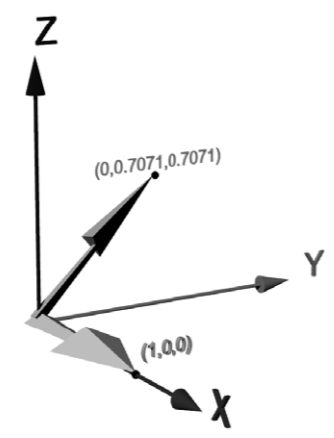
\includegraphics[width=.4\linewidth]{images/3d_start_end_rotations.png}
  \caption{Start and end rotation}
\end{subfigure}%
\begin{subfigure}{.5\textwidth}
  \centering
  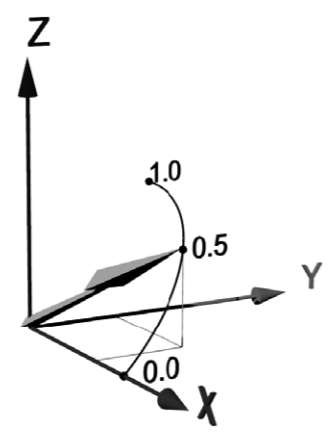
\includegraphics[width=.4\linewidth]{images/3d_interpolated_rotation.png}
  \caption{Interpolated rotation}
\end{subfigure}
\caption{3D interpolation of rotations \cite{ISO19141_moving_features}}
\label{fig:3d_interpolation}
\end{figure}

The interpolation process can be represented mathematically as follows. To interpolate between two rotations represented by quaternions \( q_0 \) and \( q_1 \), we first compute an angle \( \theta \) between them, and then apply the \textit{slerp} process to find the interpolated rotation. $r$ is a ratio value which depends on the instant of the resulting rotation, just as in \ref{section:interpolate}.

\begin{equation}
\begin{split}
    \cos(\theta)    & = q_0 \bullet q_1 \\
    q(r)            & = Slerp(q_0, q_1, r) \\
                    & = \frac{q_0 * \sin((1-r)*\theta) + q_1 * \sin(r*\theta)}{\sin(\theta)}
\end{split}
\end{equation}
    
\subsubsection{Interpolating 2d rotations using complex numbers}

We have shown how quaternions can be used to represent 3d rotations and to compute interpolation between 3d rotations. These techniques can thus also be used for 2d rotations, since they are a special type of 3d rotations and the interpolation between two 2d rotations also results in a 2d rotation. Nevertheless, using a quaternion rotation for 2d rotations might be overkill if 3d rotations do not need to be handled. A method has previously been described that handles only 2d rotations, but as said previously, it has to handle edge cases, because of the fact that rotation angles have to be between \( - \pi \) and \( \pi \). Another method uses complex numbers to, similarly to the previously mentioned quaternions, compute interpolation of 2d rotations in an efficient way. This is done using the exact same technique as with quaternions, but using less parameters. The equations are shown below, and the similarity with the previously defined equations for quaternions can clearly be seen.

A rotation of $\theta$ around the origin can be represented using the complex number \( q = \cos(\frac{\theta}{2}) + i*\sin(\frac{\theta}{2}) \) and a 2d point \( p = (x, y) \) can be represented using the complex number \( p = x + i*y \). Computing the interpolation between two rotations \( q_0 \) and \( q_1 \) can be done in a similar manner as quaternion interpolation

\begin{equation}
\begin{split}
\cos(\frac{\theta}{2})  &= q_0 \bullet q_1 \\
                        &= \cos(\frac{\theta_0}{2})*\cos(\frac{\theta_1}{2}) + \sin(\frac{\theta_0}{2})*\sin(\frac{\theta_1}{2}) \\
                        &= \cos(\frac{\theta_1 - \theta_0}{2}) \\
                        & \\
q(r)                &= Slerp(q_0, q_1, r) \\
                &= \frac{q_0 * \sin((1-r)*(\frac{\theta}{2})) + q_1 * \sin(r*(\frac{\theta}{2}))}{\sin((\frac{\theta}{2}))} \\
                &= \cos((1-r)*\frac{\theta_0}{2} + r*\frac{\theta_1}{2}) + i*\sin((1-r)*\frac{\theta_0}{2} + r*\frac{\theta_1}{2}) \\
\end{split}
\end{equation}

, and the same can be said for applying the rotation to an arbitrary point.

\begin{equation}
\begin{split}
    p'  &= q*p*q \\
        &= q^2*p \\
        &= (\cos(\frac{\theta}{2})^2 + \sin(\frac{\theta}{2})^2 + i*2\cos(\frac{\theta}{2})\sin(\frac{\theta}{2}))*p \\
        &= (\cos(\theta) + i*\sin(\theta))*(x + i*y) \\
        &= (x*\cos(\theta) - y*\sin(\theta)) + i*(x*\sin(\theta) + y*\cos(\theta)) \\
\end{split}
\end{equation}